\section{Model predictions errors for Vietnam and the United States}

When applied to data for the considered countries, namely Vietnam and the United States, both the baseline model and the second version show consistent results in predicting the trends of the disease.
Both versions were able to produce predictions that closely followed the actual numbers for shorter forecast horizons, while with longer horizons the errors quickly accumulated.
These results demonstrated the model's inability to capture the long-term dynamics of the disease even when mobility data was incorporated.
Moreover, it concluded that there was not a clear improvement in the model's performance when data from Facebook's Movement Range Maps dataset for the considered locations was included in the model.
In the case of Vietnam, both versions were able to extrapolate from the training period and predict the number of deaths with good accuracy for up to 21 days.
Furthermore, they were able to closely follow the trend in the number of cumulative cases for up to 14 days after the training period.
However, both failed to predict the sharp growth in the number of new cases as can be seen in \autoref{fig:predictions-vietnam-baseline} and \autoref{fig:predictions-vietnam-fb1}.
When trained with data for the \gls{US}, both versions produced similar results when predicting the trend of the disease as illustrated by \autoref{fig:predictions-usa-baseline} and \autoref{fig:predictions-usa-fb1}.
One noticeable difference between the results obtained from both versions after having trained with data for the \gls{US} was the number of cases where it was underestimated by the baseline model while the second version overestimated it.

% ERRORS

\begin{table}[!htb]
    \centering
    \begin{tabular}{| c | c | c | c | c | c | c| c |}
        \multirow{2}{*}{Days}
            & \multirow{2}{*}{Loc.}
            & \multicolumn{3}{c |}{Baseline}
            & \multicolumn{3}{c |}{2nd. Version} \\ \cline{3-8}
            & & MAE & MAPE & RMSE & MAE & MAPE & RMSE \\ \hline\hline

        \multirow{2}{*}{7}
            & VN & 2.409 & 4.033 & 2.470 & \textbf{2.356} & \textbf{3.943} & \textbf{2.420} \\
            & US & \textbf{727.905} & \textbf{0.116} & \textbf{834.818} & 826.050 & 0.132 & 949.121 \\ \hline

        \multirow{2}{*}{14}
            & VN & 2.222 & 3.549 & 2.321 & \textbf{2.221} & \textbf{3.540} & \textbf{2.310} \\
            & US & \textbf{1689.681} & \textbf{0.267} & \textbf{2022.840} & 1871.675 & 0.296 & 2225.024 \\ \hline

        \multirow{2}{*}{21}
            & VN & 1.743 & 2.697 & 1.969 & \textbf{1.676} & \textbf{2.609} & \textbf{1.929} \\
            & US & \textbf{2986.879} & \textbf{0.467} & \textbf{3662.566} & 3155.909 & 0.494 & 3803.063 \\ \hline

        \multirow{2}{*}{28}
            & VN & 3.530 & 4.318 & 5.408 & \textbf{3.301} & \textbf{4.062} & \textbf{5.074} \\
            & US & 4512.893 & 0.697 & 5576.519 & \textbf{4495.416} & \textbf{0.695} & \textbf{5401.567} \\ \hline
    \end{tabular}
    \caption{Out-of-sample errors of the model's predictions on the number of deaths for Vietnam and the United States. The lowest errors for each evaluation metrics at each location are highlighted.}
    \label{tab:errors-country-level-deaths}
\end{table}

According to \autoref{tab:errors-country-level-deaths}, when predicting the number of deaths for the first three forecast horizons, the baseline model showed better results on data for the \gls{US} whereas the second version of the model performed better on data for Vietnam.
With a forecast horizon of 28 days, the second version of the model achieved lower errors on both datasets.

\begin{table}[!htb]
    \centering
    \begin{tabular}{| c | c | c | c | c | c | c| c |}
        \multirow{2}{*}{Days}
            & \multirow{2}{*}{Loc.}
            & \multicolumn{3}{c |}{Baseline}
            & \multicolumn{3}{c |}{2nd. Version} \\ \cline{3-8}
            & & MAE & MAPE & RMSE & MAE & MAPE & RMSE \\ \hline\hline

        \multirow{2}{*}{7}
            & VN & 96.166 & 27.928 & 106.205 & \textbf{88.005} & \textbf{25.491} & \textbf{97.969} \\
            & US & \textbf{2006.080} & \textbf{1.343} & \textbf{2415.311} & 2051.455 & 1.370 & 2976.705 \\ \hline

        \multirow{2}{*}{14}
            & VN & 110.478 & 32.456 & 117.440 & \textbf{99.469} & \textbf{29.140} & \textbf{106.410} \\
            & US & 6775.296 & 4.326 & 8842.444 & \textbf{6004.020} & \textbf{3.849} & \textbf{7582.764} \\ \hline

        \multirow{2}{*}{21}
            & VN & 174.686 & 41.840 & 207.332 & \textbf{161.454} & \textbf{38.390} & \textbf{194.470} \\
            & US & 12426.818 & 7.766 & 16039.493 & \textbf{10781.952} & \textbf{6.974} & \textbf{14765.447} \\ \hline

        \multirow{2}{*}{28}
            & VN & 357.254 & 52.338 & 502.876 & \textbf{342.409} & \textbf{49.266} & \textbf{490.063} \\
            & US & 16943.424 & \textbf{10.771} & \textbf{21371.281} & \textbf{16516.025} & 10.859 & 21514.390 \\ \hline
    \end{tabular}
    \caption{Out-of-sample errors of the model's predictions on the number of new cases for Vietnam and the United States. The lowest errors for each evaluation metrics at each location are highlighted.}
    \label{tab:errors-country-level-new-cases}
\end{table}

When predicting the number of new cases, \autoref{tab:errors-country-level-new-cases} shows that the second version of the model had better performance on Vietnam's dataset when predicting on all four different forecast horizons.
Other cases where the baseline model performed better were with the 7-day predictions and 28-day predictions for the \gls{US}.
As previously mentioned, both versions failed to produce good predictions for the number of new cases for Vietnam with the errors calculated using \gls{MAPE} of 25\% for 7-day prediction and up to 50\% for 28-day predictions.

\begin{table}[!htb]
    \centering
    \begin{tabular}{| c | c | c | c | c | c | c| c |}
        \multirow{2}{*}{Days}
            & \multirow{2}{*}{Loc}
            & \multicolumn{3}{c |}{Baseline}
            & \multicolumn{3}{c |}{2nd. Version} \\ \cline{3-8}
            & & MAE & MAPE & RMSE & MAE & MAPE & RMSE \\
        \hline\hline

        \multirow{2}{*}{7}
            & VN & \textbf{234.690} & \textbf{2.022} & \textbf{312.078} & 241.284 & 2.081 & 313.870 \\
            & US & \textbf{39553.840} & \textbf{0.106} & \textbf{39745.361} & 61863.751 & 0.166 & 62287.404 \\ \hline

        \multirow{2}{*}{14}
            & VN & 672.504 & 5.098 & 831.731 & \textbf{643.697} & \textbf{4.894} & \textbf{785.383} \\
            & US & \textbf{30561.907} & \textbf{0.081} & \textbf{33712.852} & 88894.016 & 0.233 & 94595.820 \\ \hline

        \multirow{2}{*}{21}
            & VN & 1285.683 & 8.495 & 1645.257 & \textbf{1206.696} & \textbf{7.994} & \textbf{1533.632} \\
            & US & \textbf{71921.579} & \textbf{0.184} & \textbf{97776.403} & 132684.773 & 0.341 & 151150.555 \\ \hline

        \multirow{2}{*}{28}
            & VN & 2650.472 & 14.012 & 3786.242 & \textbf{2512.913} & \textbf{13.276} & \textbf{3605.530} \\
            & US & \textbf{137006.424} & \textbf{0.342} & \textbf{189405.400} & 210325.947 & 0.529 & 259678.415 \\ \hline
    \end{tabular}
    \caption{Out-of-sample errors of the model's predictions on the number of cumulative cases for Vietnam and the United States. The lowest errors for each evaluation metrics at each location are highlighted.}
    \label{tab:errors-country-level-total-cases}
\end{table}

Lastly, comparing the predictions errors for the number of cumulative cases of the two versions revealed that the baseline model made better predictions for the \gls{US} for all forecast horizons.
In contrast, the predictions for Vietnam made by the second version were better across different horizons except for the 7-day horizon where it performed slightly worse than the baseline model.

Overall, we can see that the baseline model performed better in some instances while in other instances, the second version performed better.
In cases where one model produced better predictions than the other, the difference in predictions errors between the models was not significant, and the differences in predictions errors can be attributed to the stochastic training process.
Hence, based on these results, mobility data did not have a positive effect on the model's predictions.

\subsection{Reproduction number and fatality rate}

Looking at \autoref{fig:R0-and-fatality-vietnam}, both versions of the model learned the same decreasing trend in the effective reproduction number and the fatality rate in Vietnam.
The reproduction number reached as high as $4.5$ with the baseline model and as high as $3.5$ with the second version at the start of the simulated period.
Both versions learned that the effective reproduction number went below $1$ at around the 20th time step.
The baseline model predicted a slightly lower fatality rate compared to the second version. At the beginning of the training period the baseline model predicted a fatality of about $0.008$, and the fatality rate decreased exponentially until the end of the simulation.

\begin{figure}[!htb]
    \centering

    \begin{subfigure}[b]{\linewidth}
        \centering
        \begin{subfigure}[b]{0.4\linewidth}
            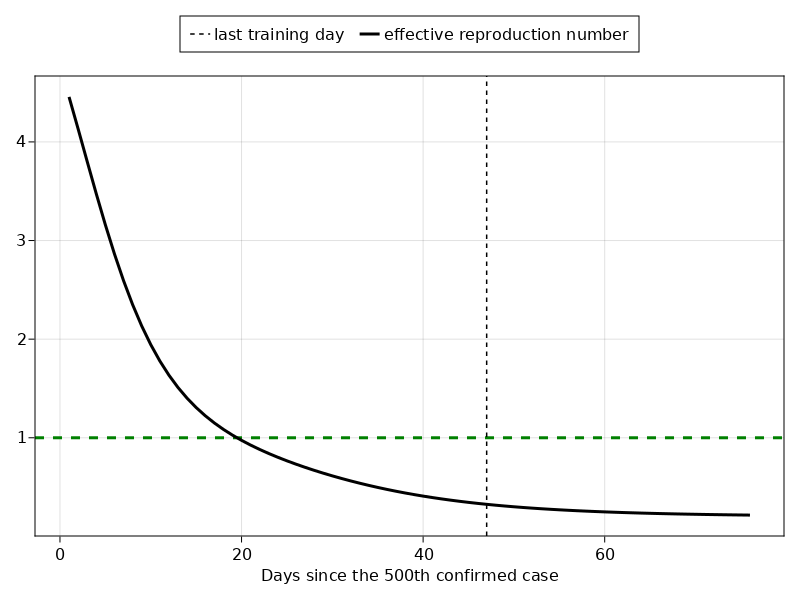
\includegraphics[width=\linewidth]{baseline/vietnam/20211216111951.baseline.vietnam.R_effective.png}
        \end{subfigure}
        \begin{subfigure}[b]{0.4\linewidth}
            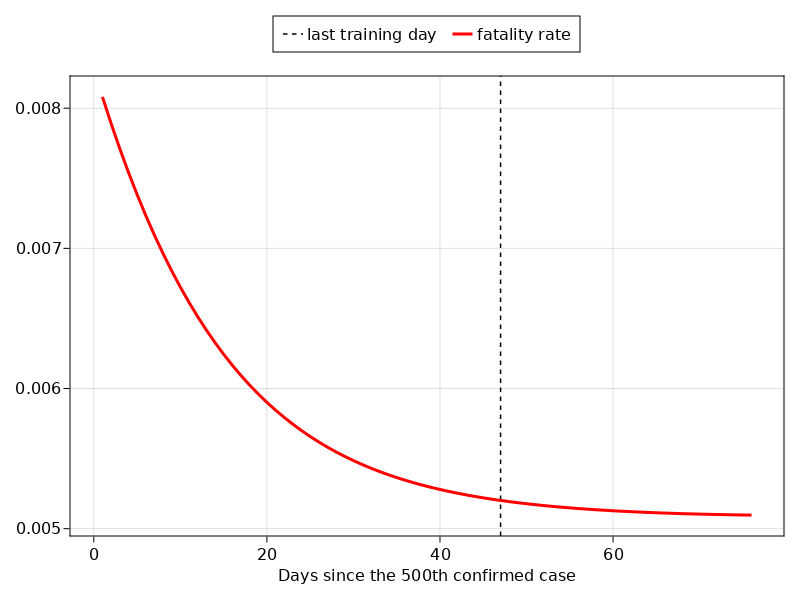
\includegraphics[width=\linewidth]{baseline/vietnam/20211216111951.baseline.vietnam.fatality_rate.png}
        \end{subfigure}
        \subcaption{Baseline model}
    \end{subfigure}

    \begin{subfigure}[b]{\linewidth}
        \centering
        \begin{subfigure}[b]{0.4\linewidth}
            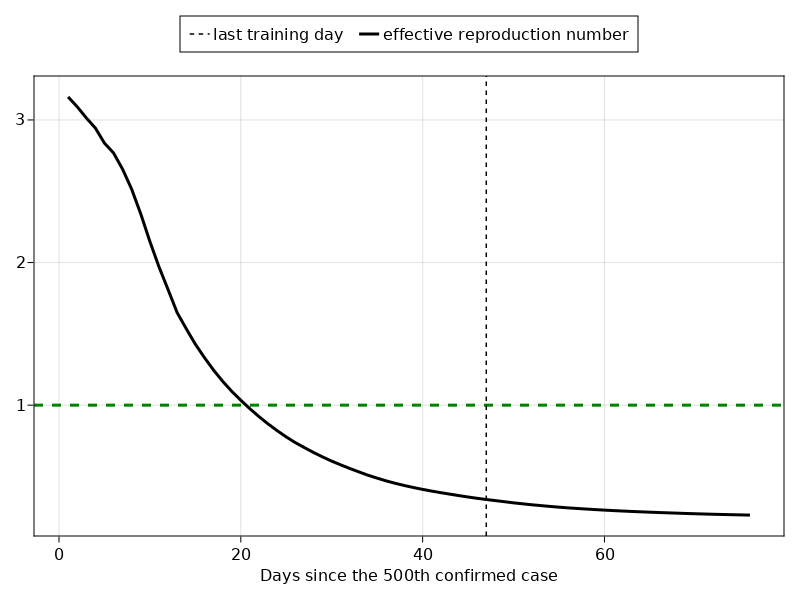
\includegraphics[width=\linewidth]{fb1/vietnam/20211216231719.fbmobility1.vietnam.R_effective.png}
        \end{subfigure}
        \begin{subfigure}[b]{0.4\linewidth}
            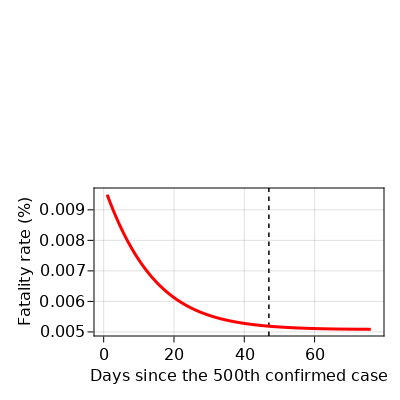
\includegraphics[width=\linewidth]{fb1/vietnam/20211216231719.fbmobility1.vietnam.fatality_rate.png}
        \end{subfigure}
        \subcaption{2nd. version}
    \end{subfigure}

    \caption{The effective reproduction number and the fatality rate for Vietnam learned by different versions of the model}
    \label{fig:R0-and-fatality-vietnam}
\end{figure}

Both versions learned the same trend of the fatality rate for the \gls{US}.
The fatality rate was at its highest of around $4.5$\% at the 0th time steps and decreased exponentially as time went on.
Then at around the 60th time step, the fatality rate was predicted to start to slowly increase.
For the effective reproduction number, the baseline model predicted the highest value of $1$ at the 0th time step, and the effective reproduction number gradually decreased until the end of the simulation.
On the other hand, the second version predicted a higher effective reproduction number of around $1.2$ at the 0th time step, and the effective reproduction number decreased for 20 time steps before it started to rise for 10 time steps and finally dying out.

\begin{figure}[!htb]
    \centering

    \begin{subfigure}[b]{\linewidth}
        \centering
        \begin{subfigure}[b]{0.4\linewidth}
            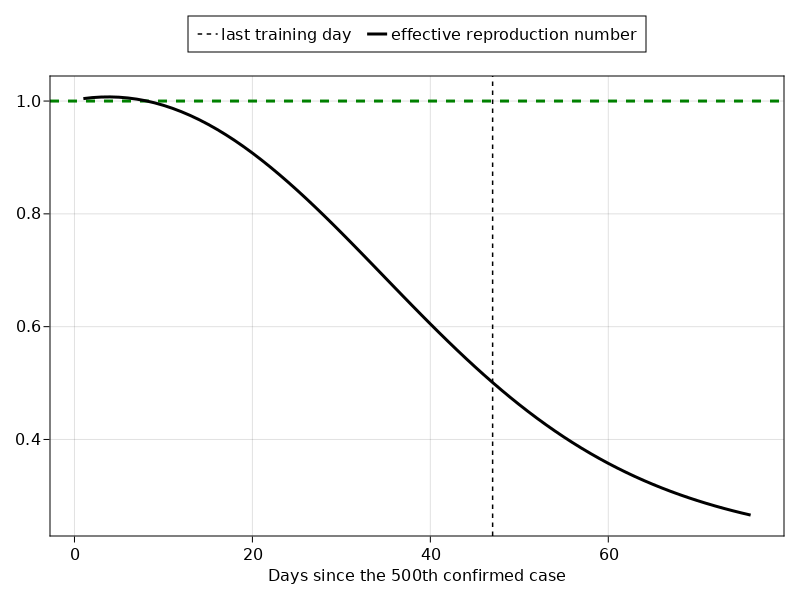
\includegraphics[width=\linewidth]{baseline/unitedstates/20211216125000.baseline.unitedstates.R_effective.png}
        \end{subfigure}
        \begin{subfigure}[b]{0.4\linewidth}
            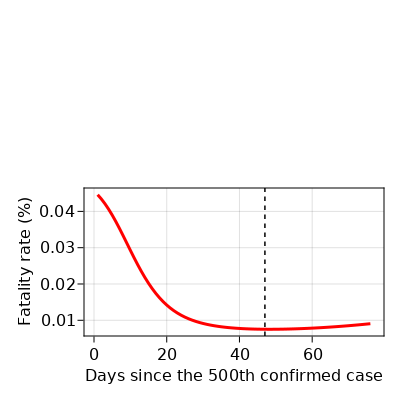
\includegraphics[width=\linewidth]{baseline/unitedstates/20211216125000.baseline.unitedstates.fatality_rate.png}
        \end{subfigure}
        \subcaption{Baseline model}
    \end{subfigure}

    \begin{subfigure}[b]{\linewidth}
        \centering
        \begin{subfigure}[b]{0.4\linewidth}
            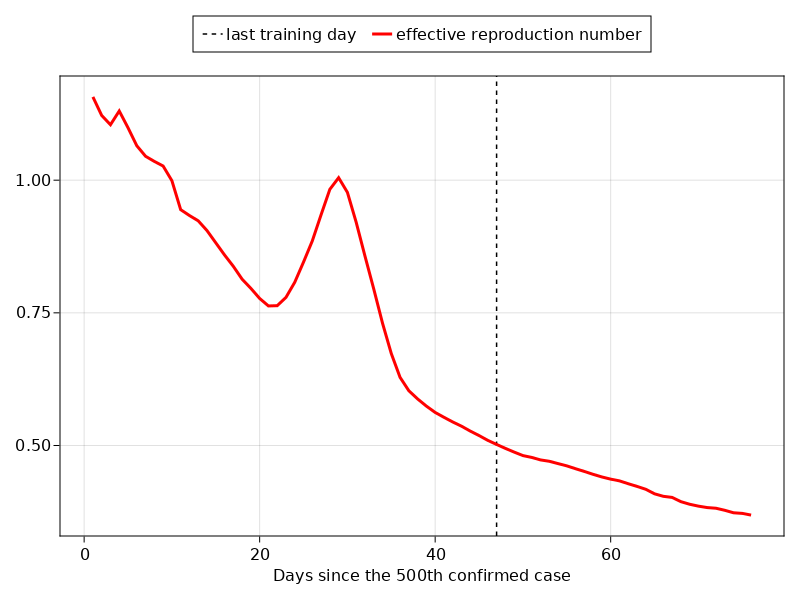
\includegraphics[width=\linewidth]{fb1/unitedstates/20211216233634.fbmobility1.unitedstates.R_effective.png}
        \end{subfigure}
        \begin{subfigure}[b]{0.4\linewidth}
            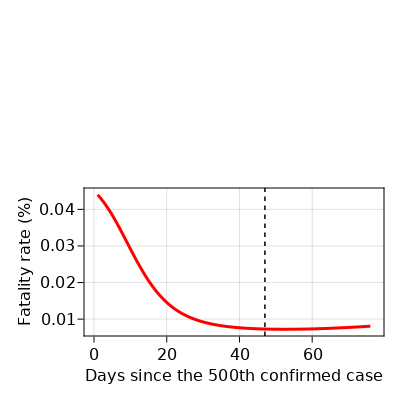
\includegraphics[width=\linewidth]{fb1/unitedstates/20211216233634.fbmobility1.unitedstates.fatality_rate.png}
        \end{subfigure}
        \subcaption{2nd. version}
    \end{subfigure}

    \caption{The effective reproduction number and the fatality rate for the United States learned by different versions of the model}
    \label{fig:R0-and-fatality-usa}
\end{figure}
